\chapter{Analisis Masalah Penangganan Kesalahan Pada \textit{Spreadsheet}}

Pada bab ini akan diuraikan analisis persoalan penangganan kesalahan pada \textit{spreadsheet} yang telah diuraikan pada Bab I. Hasil dari bab ini digunakan untuk merancang aplikasi yang akan diimplementasikan seperti yang dijelaskan pada Bab IV.

\section{Penangganan Kesalahan Pada \textit{Spreadsheet}}
Pada Subbab \ref{KesalahanPenggunaan} dijelaskan bahwa terdapat dua jenis kesalahan yang dapat terjadi pada penggunaan \textit{spreadsheet} yakni kesalahan kualitatif dan kesalahan kuantitatif. Kesalahan kualitatif merupakan kesalahan penggunaan \textit{spreadsheet} yang berhubungan dengan kualitas dan prosedur penggunaan. Contoh kesalahan kualitatif yang sering terjadi adalah penggunaan \textit{spreadsheet} sebagai basis data. Kesalahan kuantitatif merupakan kesalahan yang menyebabkan keluaran menjadi salah. Contoh kesalahan kuantitatif yang sering terjadi adalah kesalahan masukan yang tidak tervalidasi.

Pencegahan untuk kesalahan-kesalahan ini dapat dilihat pada Subbab \ref{PenangananKesalahan}. Salah satu caranya adalah pembuatan \textit{preliminary design} terhadap \textit{spreadsheet} yang dibuat. Oleh karena itu, pada aplikasi \textit{spreadsheet} yang dibangun akan langsung terhubung dengan basis data dan melalui pemeriksaan masukan saat memasukkan data. Dengan aplikasi ini diharapkan dapat menangani kesalahan kualitatif yang berupa penggunaan \textit{spreadsheet} sebagai basis data dengan cara menghubungkan \textit{spreadsheet} ke basis data yang sesungguhnya secara langsung. Serta menangani kesalahan kuantitatif dengan cara melakukan validasi masukan.

\section{Aspek Penting dalam Aplikasi \textit{Spreadsheet} Untuk Penanganan Kesalahan}
Aplikasi \textit{spreadsheet} yang baik harus dapat diakses dan digunakan secara kolaboratif yang dapat dilakukan dengan membuat aplikasi \textit{spreadsheet} tersebut berbasis \textit{web}. Aspek-aspek aplikasi \textit{web} yang perlu diperhatikan dalam membangun aplikasi \textit{spreadsheet} adalah:
\begin{enumerate}
	\item \textit{Response time}

	Membangun aplikasi berbasis \textit{web} menggunakan HTTP sebagai protokol komunikasi dan tentunya didalam komunikasi tersebut membutuhkan waktu untuk mengirimkan \textit{request} dari klien. Jika waktu yang dibutuhkan untuk melakukan respon lambat, akan sulit terjadi kolaborasi dan memperbesar kemungkinan terjadinya \textit{race condition} pada masukan pengguna. Sehingga diperlukan waktu respon yang cepat untuk dapat menangani banyak \textit{request} dalam satu waktu dan dalam waktu yang singkat.

	\item Konkurensi

	Aplikasi berbasis \textit{web} yang akan dibuat harus dapat diakses secara konkuren yakni diakses bersama-sama oleh banyak klien dalam satu waktu. Pengaksesan secara konkuren dapat berdampak pada terpanggilnya banyak \textit{query} dalam satu waktu. Oleh karena itu aplikasi yang dibuat harus dapat menjalankan secara konkuren setiap \textit{request} yang masuk.

	\item \textit{Query} basis data

	Akses terhadap basis data dibutuhkan sebagai media penyimpanan yang persisten dan konsisten. Oleh karena itu, akses terhadap basis data diperlukan untuk kemudahan penyimpanan dan pengambilan data serta mengatasi permasahalan ketidaksamaan \textit{versioning} diantara suatu \textit{file spreadsheet}.

	\item Arsitektur \textit{web}

	Aplikasi berbasis \textit{web} ini dapat diakses oleh banyak orang melalui mesin yang berbeda. Arsitektur ini juga memungkinkan untuk terpisahnya mesin penyimpanan basis data dari mesin yang berisi aplikasi utama. Dengan demikian, diperlukan aplikasi \textit{spreadsheet} yang dapat dikonfigurasi dengan mudah menurut arsitektur yang digunakan.
\end{enumerate}

Keempat aspek pada aplikasi berbasis \textit{web} tersebut akan menjadi aspek utama yang dikembangkan didalam pembuatan aplikasi \textit{spreadsheet} berbasis aplikasi \textit{web}.

Berdasarkan pada Subbab \ref{KesalahanPenggunaan}, terdapat dua jenis tipe kesalahan yang bisa terjadi pada penggunaan \textit{spreadsheet} yakni:
\begin{enumerate}
	\item Kesalahan Kualitatif

	Kesalahan kualitatif merupakan kesalahan yang berhubungan dengan kualitas yang dipengaruhi oleh prosedur pembuatan dan rancangan pada \textit{spreadsheet} tersebut. Contoh kesalahan kualitatif yang sering terjadi adalah penggunan \textit{spreadsheet} sebagai media penyimpanan atau basis data. Hal ini tidak sesuai dengan kegunaan utama dari \textit{spreadsheet} sebagai media kalkulasi dan perhitungan statistik.

	\item Kesalahan Kuantitatif

	Kesalahan kuantitatif merupakan kesalahan yang menyebabkan hasil perhitungan menjadi salah atau tidak valid. Contoh kesalahan jenis ini yang sering terjadi adalah kesalahan mekanikal dimana pengguna salah memasukan data yang tidak sesuai dengan konstrain yang ada. Hal ini dapat diatasi dengan adanya validasi sebelum data diterima. 
\end{enumerate}

Dari kedua tipe tersebut, pada Tugas Akhir ini akan lebih ditekankan kepada kesalahan kuantitatif yang bertipe kesalahan mekanikal dengan memanfaatkan teknik validasi pada masukan.

\section{Alur Proses Aplikasi \textit{Spreadsheet} Yang Akan Dibangun}
Aplikasi \textit{spreadsheet} yang dibangun terdiri dari beberapa tahap berikut yakni:
\begin{enumerate}
	\item Pengguna akan disediakan model interaksi aplikasi \textit{spreadsheet} dimana pengguna dapat membentuk struktur tempat pengguna lain memasukan input. Contohnya dalam bentuk tabel atau formulir. Pengguna juga melengkapi domain dan batasan data yang dimasukkan.
	\item Setelah pengguna selesai merancang struktur masukan, akan ditentukan bagian label dan data yang berkaitan dengan label tersebut. Bagian label dan data akan dijadikan menjadi bentuk relasional yang dapat disimpan dalam basis data
	\item Pengguna lain yang hanya memiliki kapabilitas pengisian data, hanya dapat mengisi data sesuai struktur yang diberikan. Data tersebut lalu divalidasi dan dicek kesesuaiannya sesuai dengan batasan yang diberikan sehingga memenuhi domain yang ditentukan pada basis data.
	\item Setelah proses validasi terpenuhi, data disimpan sesuai dengan relasi \textit{tuple} yang telah ditentukan. Pada saat pembukaan \textit{file spreadsheet} tersebut, akan dilakukan pemulihan data yang telah disimpan pada basis data untuk ditampilkan kembali.
\end{enumerate}

.... KASIH GAMBAR .... 

\section{Model Interaksi Pengguna}
Di dalam pembangunan perangkat lunak \textit{spreadsheet} untuk mengurangi kesalahan, dapat diidentifikasikan dua model interaksi yang dapat diimplementasi. Model interaksi yang pertama adalah menggunakan formulir sebagai basis masukan data dan model yang kedua adalah menggunakan aplikasi \textit{spreadsheet} secara langsung sebagai media input data.
	\subsection{Berbasis Formulir}
	Model interaksi ini menggunakan \textit{spreadsheet} sebagai tempat perancangan formulir. Pembuat formulir akan menentukan area label dan input secara manual serta diidentifikasikan berdasarkan warna atau properti lain yang unik pada sel tersebut. Formulir akan dibangkitkan oleh aplikasi agar menjadi bentuk HTML dan terhubung ke basis data. Pengisian data oleh pengguna dilakukan melalui formulir yang dibangkitkan dan dapat diakses melalui web. Beberapa cara dapat dilakukan untuk mengimplementasikan teknik ini antara lain, mengembangkan dari aplikasi \textit{spreadsheet} yang telah ada menggunakan \textit{plugin} atau membuat aplikasi baru yang dapat melakukan konversi otomatis menjadi formulir.

	\subsection{Berbasis \textit{Spreadsheet}}
	Model interaksi berbasiskan \textit{spreadsheet} menggunakan antarmuka yang telah disediakan oleh aplikasi. Penggunaannya dilakukan dengan membuat format pengisian seperti membuat tabel pada \textit{spreadsheet} pada umumnya. Pada tabel harus terdapat label dan data sehingga metadata minimal yang dibutuhkan dapat dicapai. Fitur-fitur yang ada pada \textit{spreadsheet} juga tetap dapat digunakan saat pembuatan tabel yang diinginkan. Dari pembuatan tabel tersebut dilakukan identifikasi label dari data tersebut untuk selanjutnya diproses melalui penyaringan masukan dan dimasukan ke tabel yang sesuai yang ada di basis data. Untuk mengimplementasikan teknik ini harus mengubah kode pada program \textit{spreadsheet} atau mengekstensi fitur yang ada menggunakan \textit{plugin}. 

	\subsection{Perbandingan Model Interaksi}
	Kedua model interaksi tersebut memiliki beberapa perbedaan dan efek terhadap penggunaannya baik bagi sistem maupun pengguna. Pada Tabel \ref{ModelInteraksi} dijabarkan perbandingan antara kedua model interaksi tersebut.

	\begin{longtable}{ | p{3cm} | p{4cm} | p{4cm} | }
	    \caption{Perbandingan Model Interaksi}
	    \label{ModelInteraksi}\\ \hline
	    \centering\bfseries{Parameter} & \centering\bfseries{Berbasis Formulir} & \centering\bfseries{Berbasis \textit{Spreadsheet}} \tabularnewline \hline
	    \endfirsthead
	    \hline
	    \centering\bfseries{Parameter} & \centering\bfseries{Berbasis Formulir} & \centering\bfseries{Berbasis \textit{Spreadsheet}} \tabularnewline \hline
	    \endhead
	    Fungsionalitas & Berhasil memisahkan bagian operasional dan data. Pengguna hanya memodifikasi dan melakukan input pada bagian data. Bagian operasional hanya dapat dimodifikasi oleh pembuat formulir tersebut. & Jika tidak menggunakan proteksi terhadap sel yang dapat ditulis, tidak terjadi pemisahan antara data dan operasional sehingga beberapa kesalahan yang terjadi pada saat input masih dapat terjadi. \\ \hline
	    Teknologi & Dibutuhkan adanya algoritma tambahan untuk menangani formulir dan masukannya, serta melakukan konversi dan \textit{parsing} dari sel pada \textit{spreadsheet} ke dalam bentuk formulir. & Dibutuhkan algoritma dan logika \textit{parsing} yang lebih detil dan kompleks dalam menangani kasus-kasus table tertentu. \\ \hline
	    Antarmuka & Menggunakan antarmuka formulir yang kaku terurut dari atas ke bawah serta tidak dapat melihat hasil masukan secara langsung. & Struktur tabel atau masukan dapat disesuaikan dengan kebutuhan dan tidak perlu mempelajari hal lain jika sebelumnya telah menggunakan \textit{spreadsheet} sebagai media untuk memasukan data. \\ \hline
  	\end{longtable}

  	... dijelasin kenapa jadinya milih mana ...

\section{Penentuan Bagian Data dan Label}
Pada pembuatan \textit{spreadsheet} pada umumnya, didapatkan bahwa kebanyakan \textit{spreadsheet} pada umumnya berbentuk tabel yang terdiri dari dua unsur utama yakni data dan label atau disebut juga tipe \textit{data frame} \parencite{Chen2013}. Bagian data merupakan bagian yang biasanya dinamis dan merupakan masukan pengguna. Bagian label merupakan bagian yang memberikan keterangan dan konteks mengenai data yang dimaksud. Pada Gambar \ref{DataFrameSederhana} dapat dilihat bahwa area dengan nomor 1 disebut sebagai label yang menjelaskan data-data dibawahnya yakni pada area nomor 2.

\begin{figure}[htb]
    \centering
    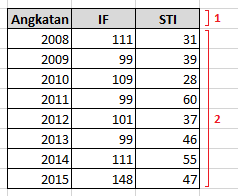
\includegraphics[width=0.3\textwidth]{resources/chapter-3-simple-dataframe.png}
    \caption{Contoh \textit{Data Frame} Sederhana}
	\label{DataFrameSederhana}
\end{figure}

	\subsection{Secara Manual oleh Pengguna}
	Penentuan label dan data dilakukan oleh pengguna secara langsung saat pembuatan tabel. Pengguna sendiri yang menentukan area mana yang merupakan label dan data mana yang dijelaskan oleh label tersebut. Dengan metode manual ini, pengguna dapat menyesuaikan bentuk tabel sesuai keinginan mereka. Metode ini menyerahkan sepenuhnya tanggungjawab keterhubungan sel label dan sel data kepada pengguna.

	\subsection{Secara Otomatis}
	Pencarian label dan data dapat menggunakan algoritma seperti yang telah dijelaskan pada Subbab \ref{metodepencarian}. Mekanisme untuk mengidentifikasi label dan data dapat dilakukan melalui 3 tahapan yakni, \textit{frame finder}, \textit{hierarchy extractor}, dan \textit{tuple builder}. Pada tahap pertama yakni \textit{frame finder} bertujuan untuk mengidentifikasi wilayah nilai (data) dan wilayah atribut (label) yang dapat berupa \textit{left attribute} maupun \textit{top attribute}. Tahap selanjutnya adalah \textit{hierarchy extractor} bertujuan untuk mendapatkan hirarki dari atribut-atribut yang ada sehingga label yang tertulis dapat dicari keterhubungan dan konteksnya terhadap data yang ada. Tahap terakhir adalah \textit{tuple builder} yang mentrasformasikan data dan label tersebut dalam bentuk \textit{tuple} yang dapat diterima oleh basis data relasional.

	\subsection{Perbandingan Metode Penentuan}
	Untuk mengetahui perbandingan kedua metode, pada Tabel \ref{centering} dijelaskan kelebihan dan kekurangan dua metode yang telah disebutkan sebelumnya.
	\begin{longtable}{ | p{3cm} | p{4cm} | p{4cm} | }
	    \caption{Perbandingan Metode Penentuan Data dan Label}
	    \label{MetodePenentuan}\\ \hline
	    \centering\bfseries{Keterangan} & \centering\bfseries{Manual oleh Pengguna} & \centering\bfseries{Otomatis} \tabularnewline \hline
	    \endfirsthead
	    \hline
	    \centering\bfseries{Keterangan} & \centering\bfseries{Manual oleh Pengguna} & \centering\bfseries{Otomatis} \tabularnewline \hline
	    \endhead
	    Kelebihan & Tingkat akurasi lebih tinggi karena data dan label yang ditentukan sesuai dengan keinginan pengguna. & Kenyamanan dalam penggunaan karena pengguna tidak perlu melakukan interferensi tambahan. Selain itu, sistem kemungkinan data dan label yang diambil dapat diubah ke dalam bentuk \textit{tuple} relasional lebih tinggi. \\ \hline
	    Kekurangan & Interferensi pengguna yang banyak dan mungkinnya data dan label tidak dapat dijadikan bentuk \textit{tuple} relasional. & Algoritma ini hanya optimal jika digunakan pada tabel yang terurut vertikal. \\ \hline
  	\end{longtable}
  	Dari perbandingan diatas, dapat dilihat terdapat kekurangan dan kelebihan didalam menggunakan salah satu metode tersebut. Berdasarkan hal tersebut, yang akan dipilih sebagai metode penentuan data dan label adalah gabungan dari kedua metode tersebut. Sistem awalnya akan melakukan \textit{parsing} terhadap struktur yang telah dibuat oleh pengguna, kemudian pengguna dapat melihat hasil dari \textit{parsing} tersebut sehingga pengguna dapat memperbaiki jika terdapat hasil pelabelan yang salah. Dengan metode gabungan ini diharapkan dapat meningkatkan akurasi dan mengurangi kesalahan \textit{parsing} yang terjadi namun tetap memberikan kenyamanan terhadap pengguna serta menjaga agar hasil pelabelan tetap dapat diubah ke dalam bentuk \textit{tuple} relasional.

\section{Pengecekan Data}
Setelah pengguna memasukan datanya kedalam struktur yang telah ditetapkan, pengecekan data dilakukan. Tujuan dari mekanisme ini adalah untuk menghindari kesalahan masukan yang terjadi dan menyesuaikan tipe yang diterima oleh tabel pada basis data. Contohnya, data masukan yang seharusnya berupa \textit{integer} menerima masukan berupa \textit{string}, sistem akan melakukan validasi dan menolak data masukan sehingga pengguna dapat memperbaiki data. Selain melakukan pengecekan terhadap tipe data, validasi juga melakukan pengecekan terhadap domain masukan. Contohnya, pengguna dapat juga mengatur rentang \textit{integer} yang boleh dijadikan masukan atau \textit{string} apa saja yang dapat diterima oleh sistem.

\section{Penyimpanan dan Pemulihan Data}
Data yang telah dimasukan oleh pengguna baik data bentuk struktur \textit{spreadsheet} maupun data masukan pada struktur disimpan ke dalam basis data yang presisten. Hasil dari pendeteksian label dan data akan diubah menjadi \textit{tuple} relasional yang dapat diterima oleh basis data relasional. Contoh pengubahan yang terjadi dapat dilihat pada Gambar \ref{RelationalTuple} yang diilustrasikan oleh Chen tahun 2013 pada \textit{paper} mengenai Senbazuru.

\begin{figure}[htb]
    \centering
    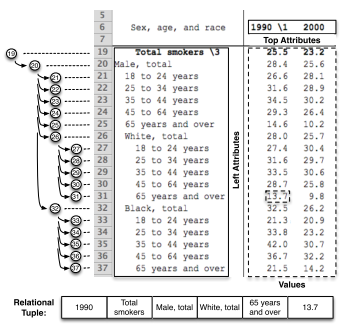
\includegraphics[width=0.6\textwidth]{resources/chapter-3-relational-tuple.png}
    \caption{Contoh \textit{Tuple} Relasional \parencite{Chen2013}}
	\label{RelationalTuple}
\end{figure}

Setelah data dan label dijadikan \textit{tuple} relasional, \textit{tuple} dimasukan ke dalam basis data dengan menggunakan operasi \textit{insert} ke dalam tabel yang terhubung dengan data tersebut. Pada saat pemulihan data, data yang disimpan akan kembali ditampilkan pada sel yang bersesuaian sehingga pengguna dapat melanjutkan perubahan pada \textit{spreadsheet} dan berkolaborasi.
